\chapter{Конструкторская часть}

\section{Требования к программному обеспечению}
Программа должна предоставлять пользователю графический интерфейс, позволяющий:
\begin{itemize}
	\item загрузить исходный и целевой объект из \textit{.obj} файла;
	\item выбрать цвет и оптические свойства поверхности загруженных объектов;
	\item просматривать каждый объект и результат морфинга посредством поворота и масштабирования;
	\item изменять масштабирование и поворот исходного и целевого объектов морфинга;
	\item выбирать стадию морфинга объектов.
\end{itemize}

Программа должна корректно реагировать на любые действия пользователя.

\section{Используемы типы и структуры данных}
\begin{enumerate}
	\item[1)] Сцена состоит из:
	\begin{itemize}
		\item объекта;
		\item камеры;
		\item источника света.
	\end{itemize}
	
	\item[2)] Объект состоит из:
	\begin{itemize}
		\item массива точек;
		\item массива треугольников (индексы вершин);
		\item массива внешних нормалей к треугольникам;
		\item материала;
		\item матрицы преобразований.
	\end{itemize}
	
	\item[3)] Результат морфинга, состоит из:
	\begin{itemize}
		\item массива точек;
		\item массива функций, интерполирующих вершины в момент $t$;
		\item массива треугольников (индексы вершин);
		\item массива внешних нормалей к треугольникам;
		\item массива функций, интерполирующих внешние нормали в момент $t$;
		\item материала;
		\item функции интерполирующей материал в момент $t$;
		\item матрицы преобразований.
	\end{itemize}
	
	\item[4)] камера состоит из:
	\begin{itemize}
		\item положения;
		\item точки, на которую направлен взгляд;
		\item угол обзора в радианах;
		\item отношение сторон;
		\item уаление ближней плоскости пирамиды видимости;
		\item удаление дальней плоскости пирамды видимости.
	\end{itemize}
	
	\item[5)] источник света состоит из:
	\begin{itemize}
		\item положения;
		\item интесивности;
		\item цвета; TODO: возможно убрать
	\end{itemize}
	
	\item[6)] материал состоит из:
	\begin{itemize}
		\item цвета в формате \textit{RGB};
		\item коэффициента диффузного отражения;
		\item коэффициента зеркального отражения;
		\item степени, аппроксимирующей пространственное распределение зеркально отраженного света.
	\end{itemize}
\end{enumerate}

Для построения суперсетки используется структура данных DCEL (doubly connected edge list)~\cite{alexa}. Визуальное представление структуры данных приведено на рисунке~\ref{fig:DCEL}.

\begin{figure}[H]
	\centering
	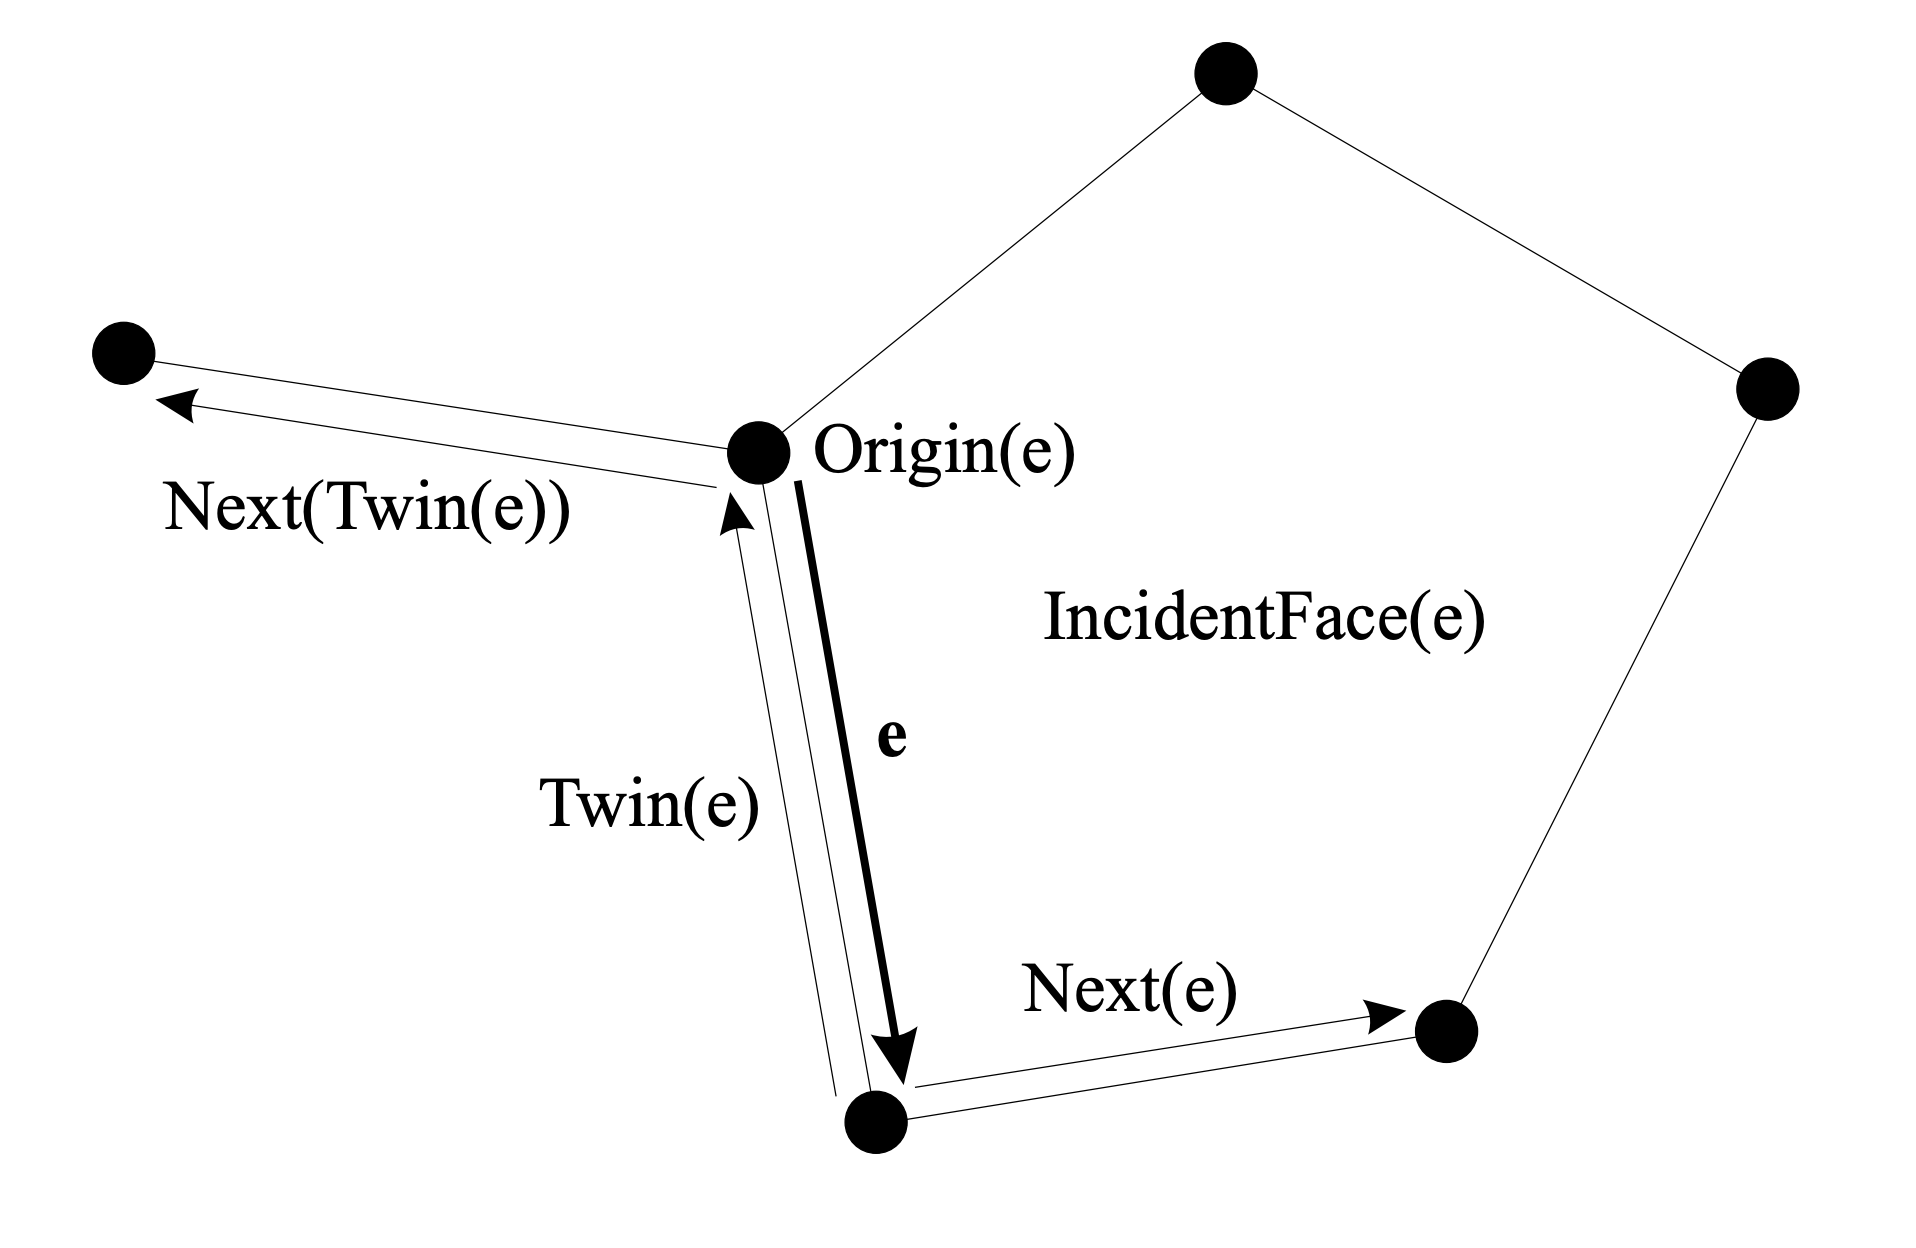
\includegraphics[width=0.5\textwidth]{DCEL}
	\label{fig:DCEL}
	\caption{DCEL (doubly connected edge list)~\cite{alexa}}
\end{figure}

DCEL состоит из:

\begin{itemize}
	\item массив вершин;
	\item массив полуребер;
	\item массив граней;
\end{itemize}

Полуребро состоит из:
\begin{itemize}
	\item индекса вершины-начала;
	\item индекса полуребра-двойника;
	\item индекса смежной грани;
	\item индекса следующего полуребра;
\end{itemize}

Грань состоит из индекса полуребра, связанного с ней.

\section{Математические основы алгоритмов}

\subsection{Барицентрические координаты}

Барицентрические координаты $\alpha$, $\beta$ и $\gamma$ определяют положение точки $P$ относительно вершин треугольника $A$, $B$ и $C$~\cite{foley}.

Точка $P$ находится внутри или на границах треугольника $ABC$, если она может быть представлена в виде аффинной комбинации вершин~\cite{foley}:
\begin{equation}
	P = \alpha A + \beta B + \gamma C \text{, где } \alpha + \beta + \gamma = 1, \text{ и } \alpha, \beta, \gamma \geq 0 \text{\cite{foley}}
\end{equation}

Если хотя бы одна из координат $\alpha, \beta, \gamma$ отрицательна, то точка $P$ лежит вне треугольника~\cite{foley}.

Барицентрическая координата $\alpha$ точки $P$ пропорциональна площади треугольника $PBC$ (см. рисунок~\ref{fig:barycentric}) (треугольника, противолежащего вершине $A$)~\cite{foley}.

\begin{figure}[H]
	\label{fig:barycentric}
	\centering
	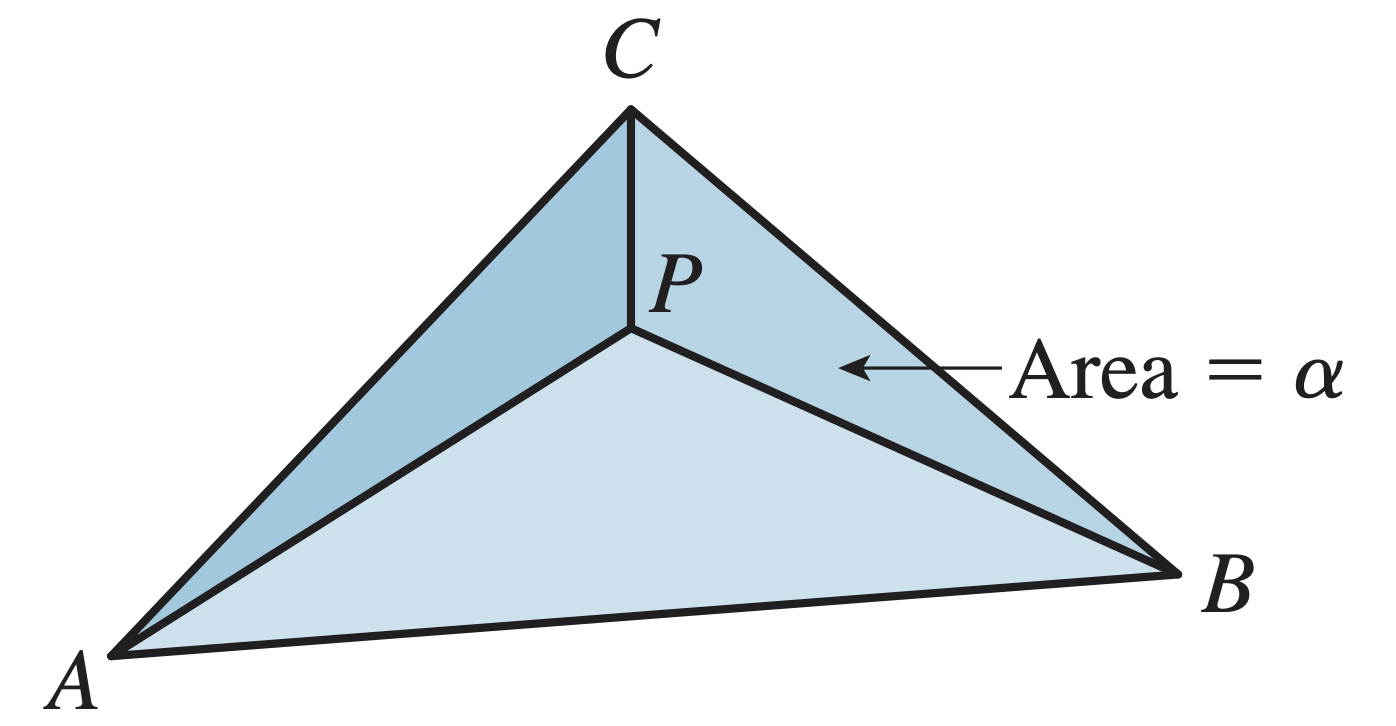
\includegraphics[width=0.5\textwidth]{barycentric_coordinates}
	\caption{Точка $P$ разделяет треугольник $ABC$ на три меньших треугольника, площади которых соотносятся как $\alpha$, $\beta$ и $\gamma$; Барицентрические координаты точки $P$ равны ($\alpha$, $\beta$, $\gamma$)~\cite{foley}}
\end{figure}

Координата $\alpha$ точки $P$ определяется как отношение площади треугольника $PBC$ к площади всего треугольника $ABC$~\cite{foley}:

\begin{equation}
	\alpha = \frac{S_{\triangle PBC}}{S_{\triangle ABC}}
\end{equation}

Аналогичные соотношения используются для $\beta$ (пропорционально $S_{\triangle PAC}$) и $\gamma$ (пропорционально $S_{\triangle PAB}$).

На плоскости барицентрические координаты точки $P$ в треугольнике $ABC$ могут быть вычислены при помощи косого произведения:

\begin{equation}
	\begin{aligned}
		\begin{cases}
		\alpha = \frac{|BC \times BP|}{|AB \times AC|} = \frac{(C - B)_x \cdot (P - B)_y - (C - B)_y \cdot (P - B)_x}{(B - A)_x \cdot (C - A)_y - (B - A)_y \cdot (C - A)_x} \\
		\beta = \frac{|CA \times CP|}{|AB \times AC|} = \frac{(A - C)_x \cdot (P - C)_y - (A - C)_y \cdot (P - C)_x}{(B - A)_x \cdot (C - A)_y - (B - A)_y \cdot (C - A)_x} \\
		\gamma = 1 - \alpha - \beta
		\end{cases}
	\end{aligned}
\end{equation}

\subsection{Поиск пересечения дуг на единичной сфере}

Для нахождения пересечения дуг необходимо:
\begin{enumerate}
	\item[1)] найти прямую по которой пересекаются плоскости, содержащие дуги;
	\item[2)] найти точки пересечение прямой с единичной сферой;
	\item[3)] проверить принадлежность точек обеим дугам.
\end{enumerate}

Пусть дуга $A$ ограничена точками $A_0$, $A_1$, а дуга $B$ --- $B_0$, $B_1$.

Направляющий вектор прямой можно вычислить как векторное произведение нормалей к плоскостям, содержащим дуги:

\begin{equation}
	\mathbf{d} = \mathbf{n_A} \times \mathbf{n_B} = (\mathbf{A_0} \times  \mathbf{A_1}) \times (\mathbf{B_0} \times  \mathbf{B_1})
\end{equation}

Точки пересечения с единичной сферой равны:

\begin{equation}
	P_{1,2} = \pm \frac{\mathbf{d}}{\parallel\mathbf{d}\parallel}
\end{equation}

Т.~к. длина радиус-векторов всех точек на единичной сфере равна 1, скалярное произведение равно косинусу угла между векторами. В таком случае точка $P_{1,2}$ принадлежит обеим дугам $A$ и $B$, а следовательно является их пересечением если:

\begin{equation}
	\begin{cases}
		A_0 \cdot A_1 \le A_0 \cdot P_{1,2}\\
		A_0 \cdot A_1 \le A_1 \cdot P_{1,2}\\
		B_0 \cdot B_1 \le B_0 \cdot P_{1,2}\\
		B_0 \cdot B_1 \le B_1 \cdot P_{1,2}
	\end{cases}
\end{equation}

\section{Описание алгоритмов}

\begin{figure}[H]
	\label{fig:morphig_idef0}
	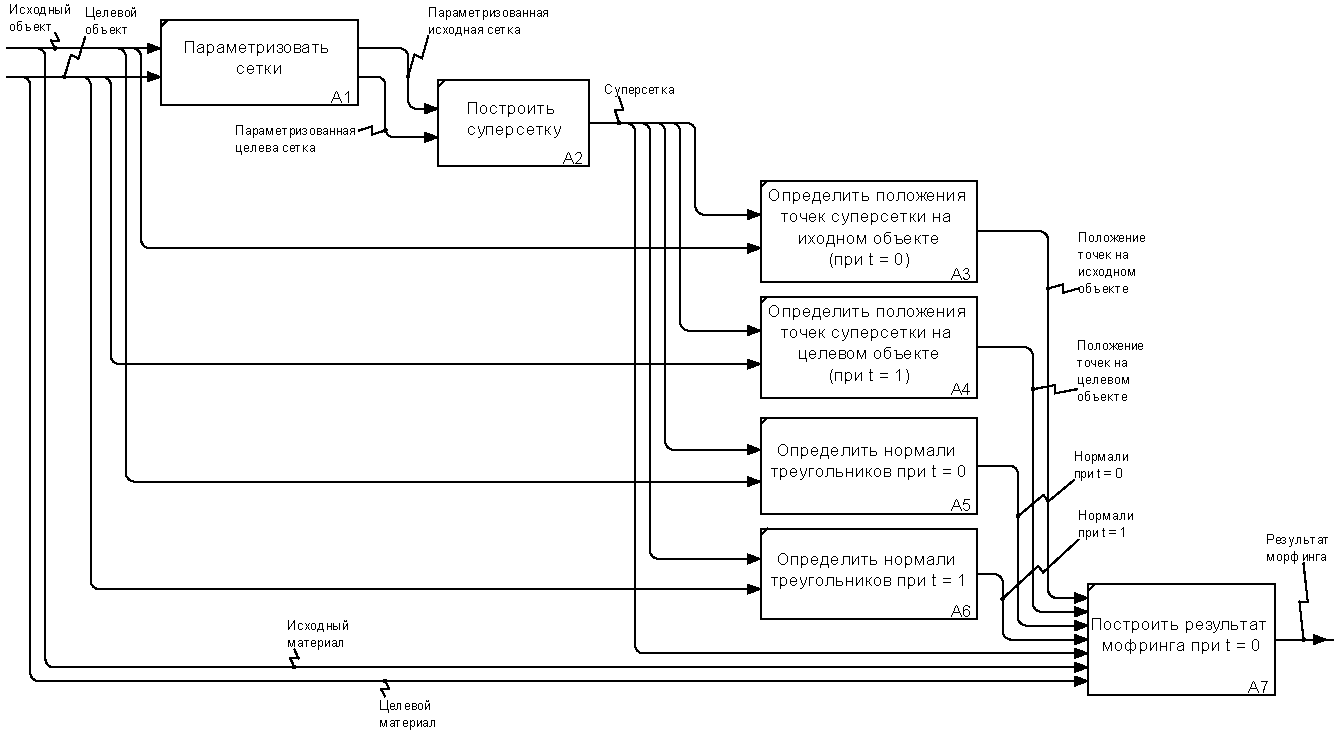
\includegraphics[width=\textwidth]{morphing_idef0}
	\caption{Функциональная модель построения морфинга}
\end{figure}

Схемы основных алгоритмов, используемых в программном обеспечены представлены на рисунках~\ref{fig:flowсhart_z-buff}--\ref{fig:flowсhart_vertex_relocation}.

\begin{figure}[H]
	\label{fig:flowсhart_z-buff}
	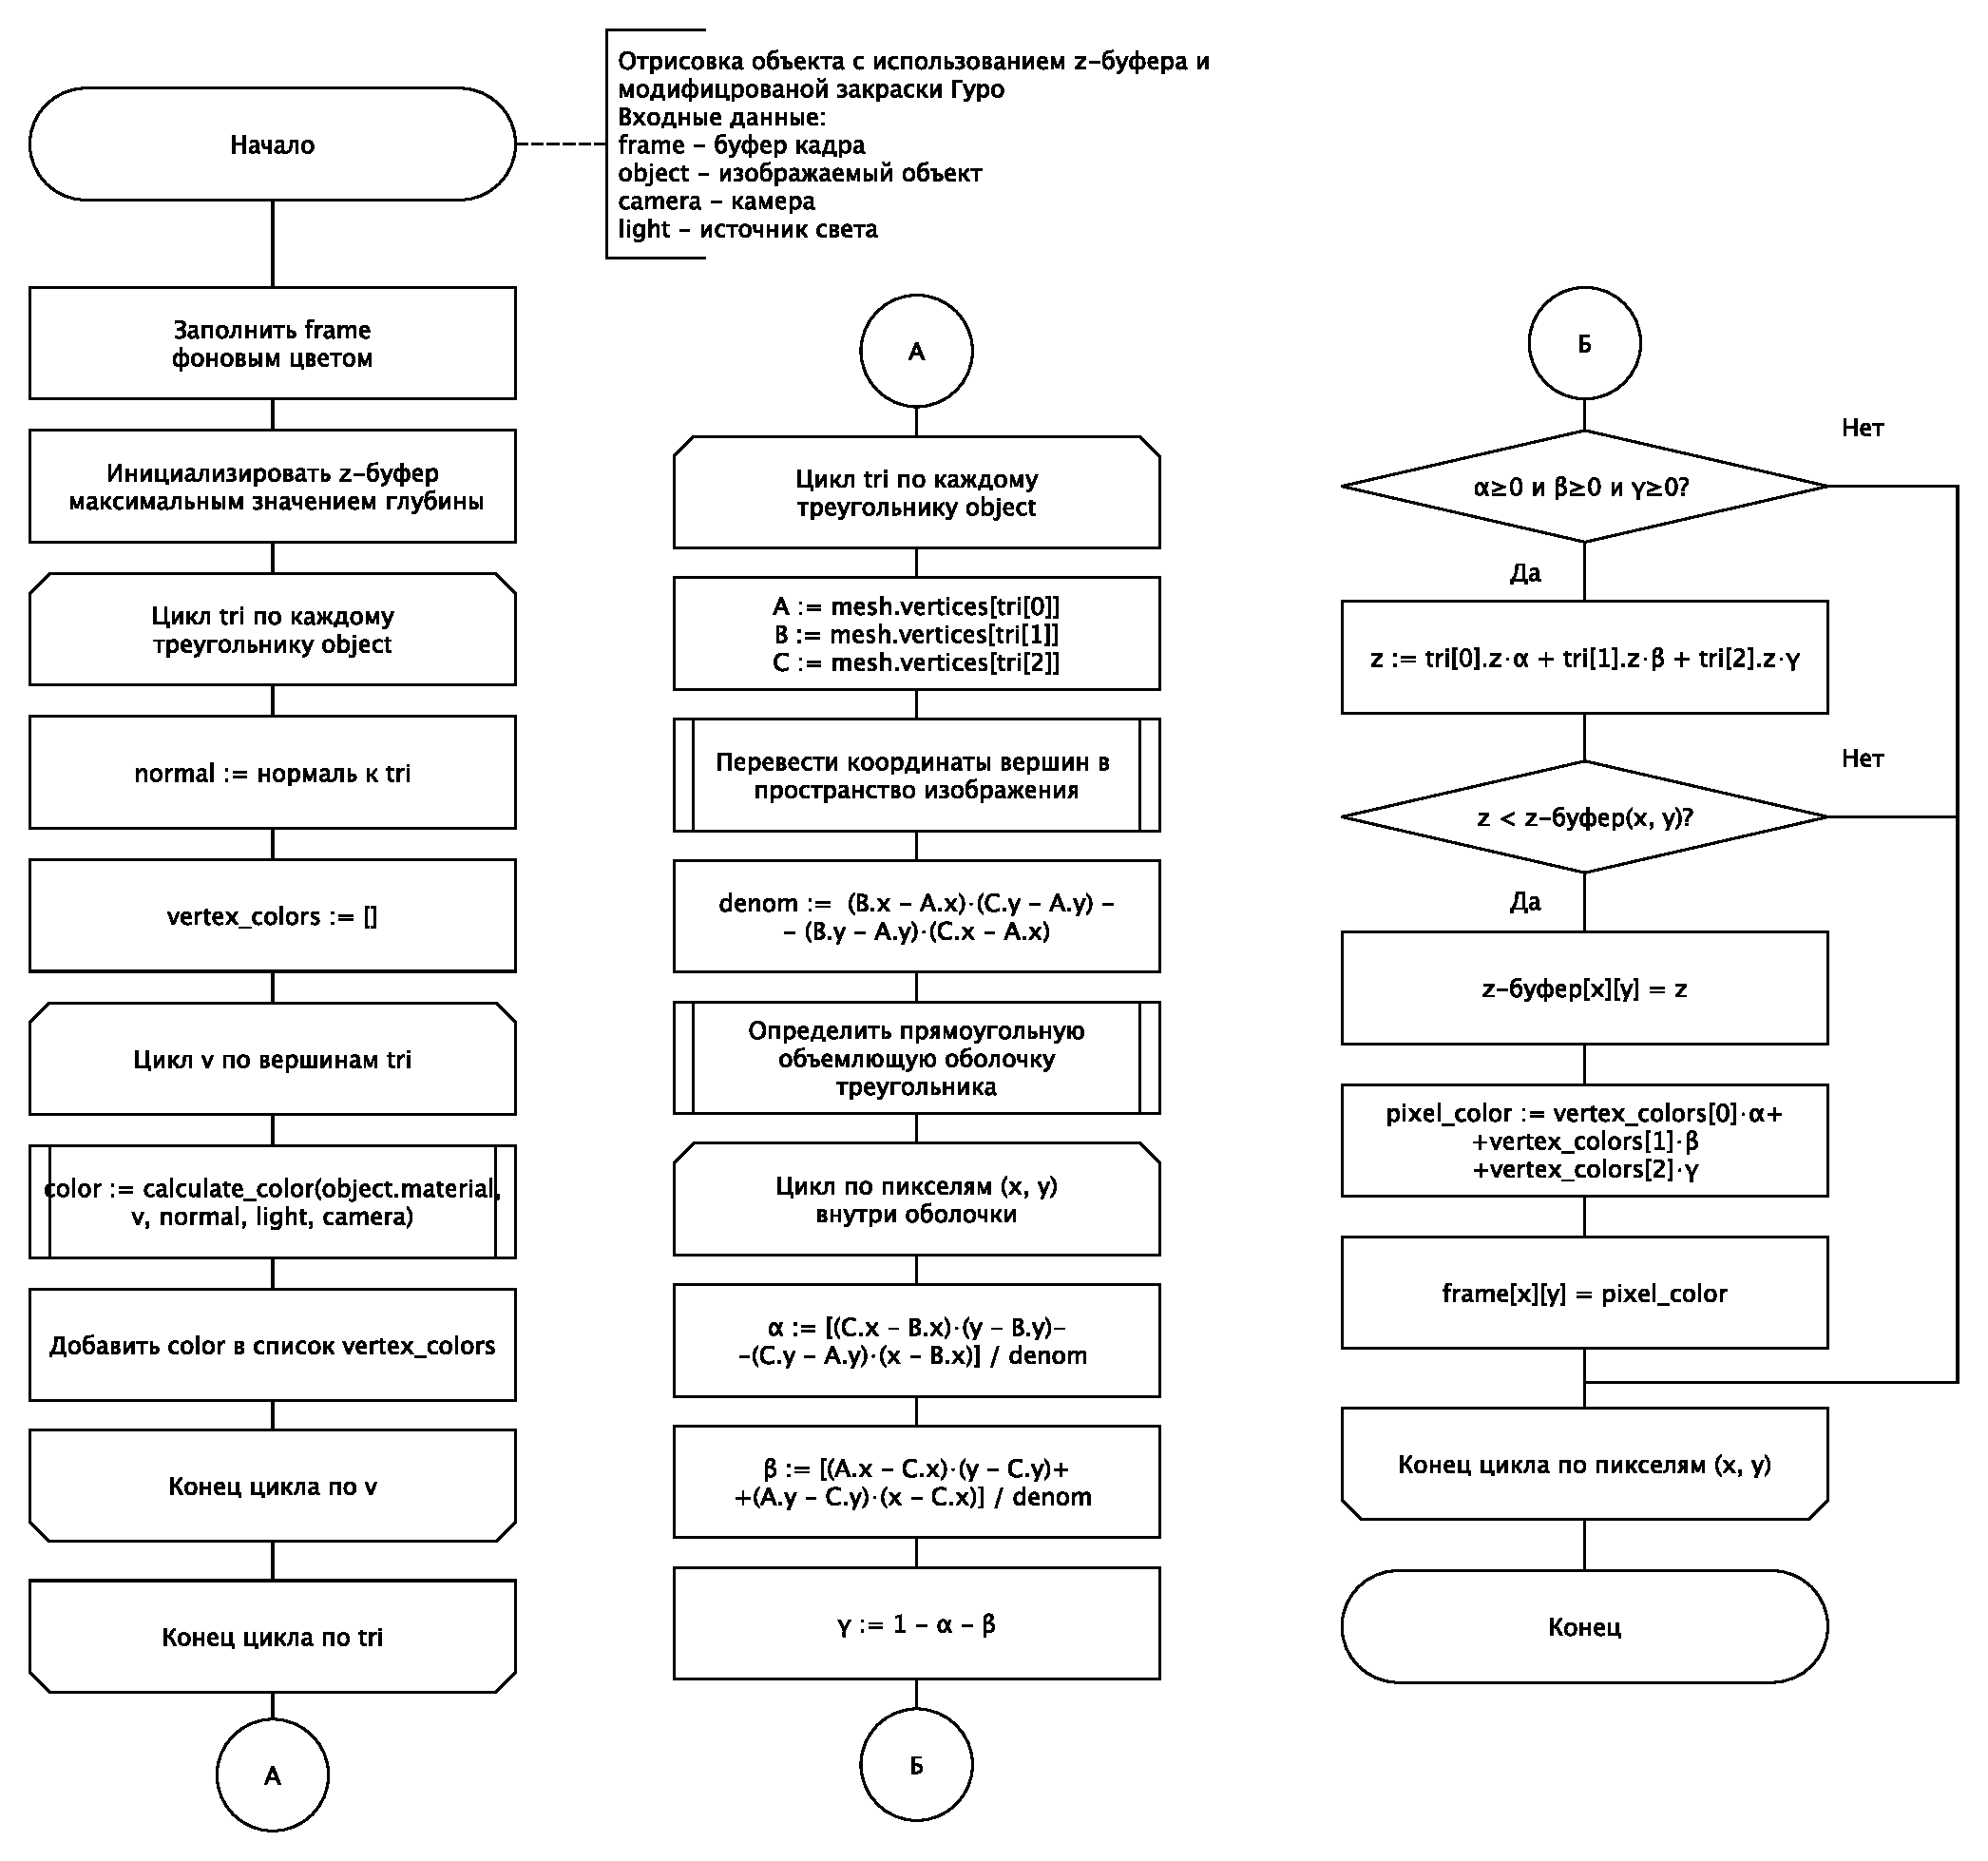
\includegraphics[width=\textwidth]{flowchart_z-buff}
	\caption{Схема алгоритма отрисовки объекта с использованием \textit{z}-буфера и модифицированной закраски Гуро}
\end{figure}

\begin{figure}[H]
	\label{fig:flowсhart_parametrization}
	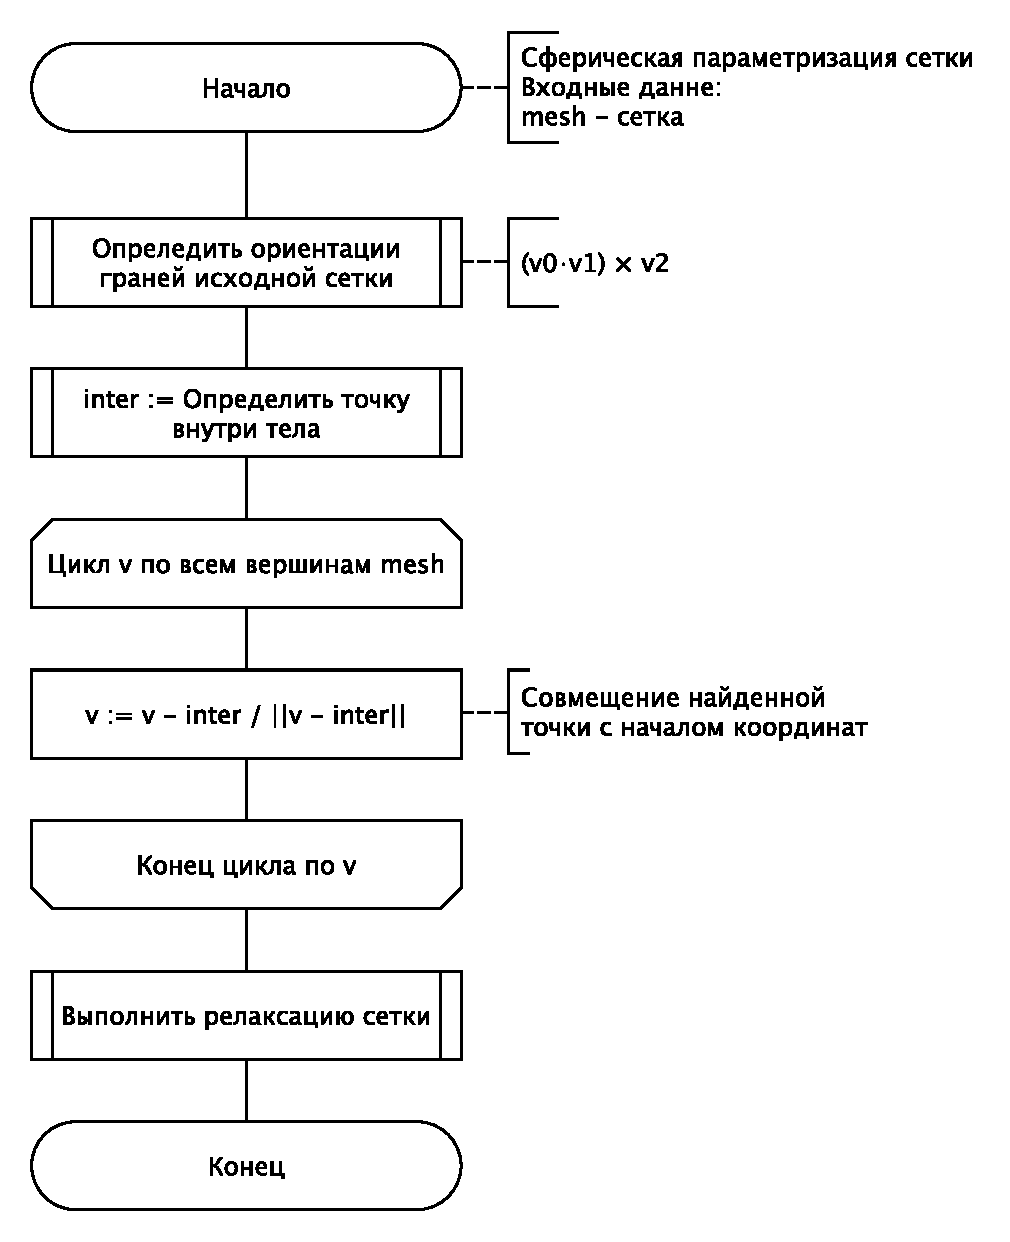
\includegraphics[width=\textwidth]{flowchart_parametriztion}
	\caption{Схема алгоритма сферической параметризации сетки}
\end{figure}

\begin{figure}[H]
	\label{fig:flowсhart_relaxation}
	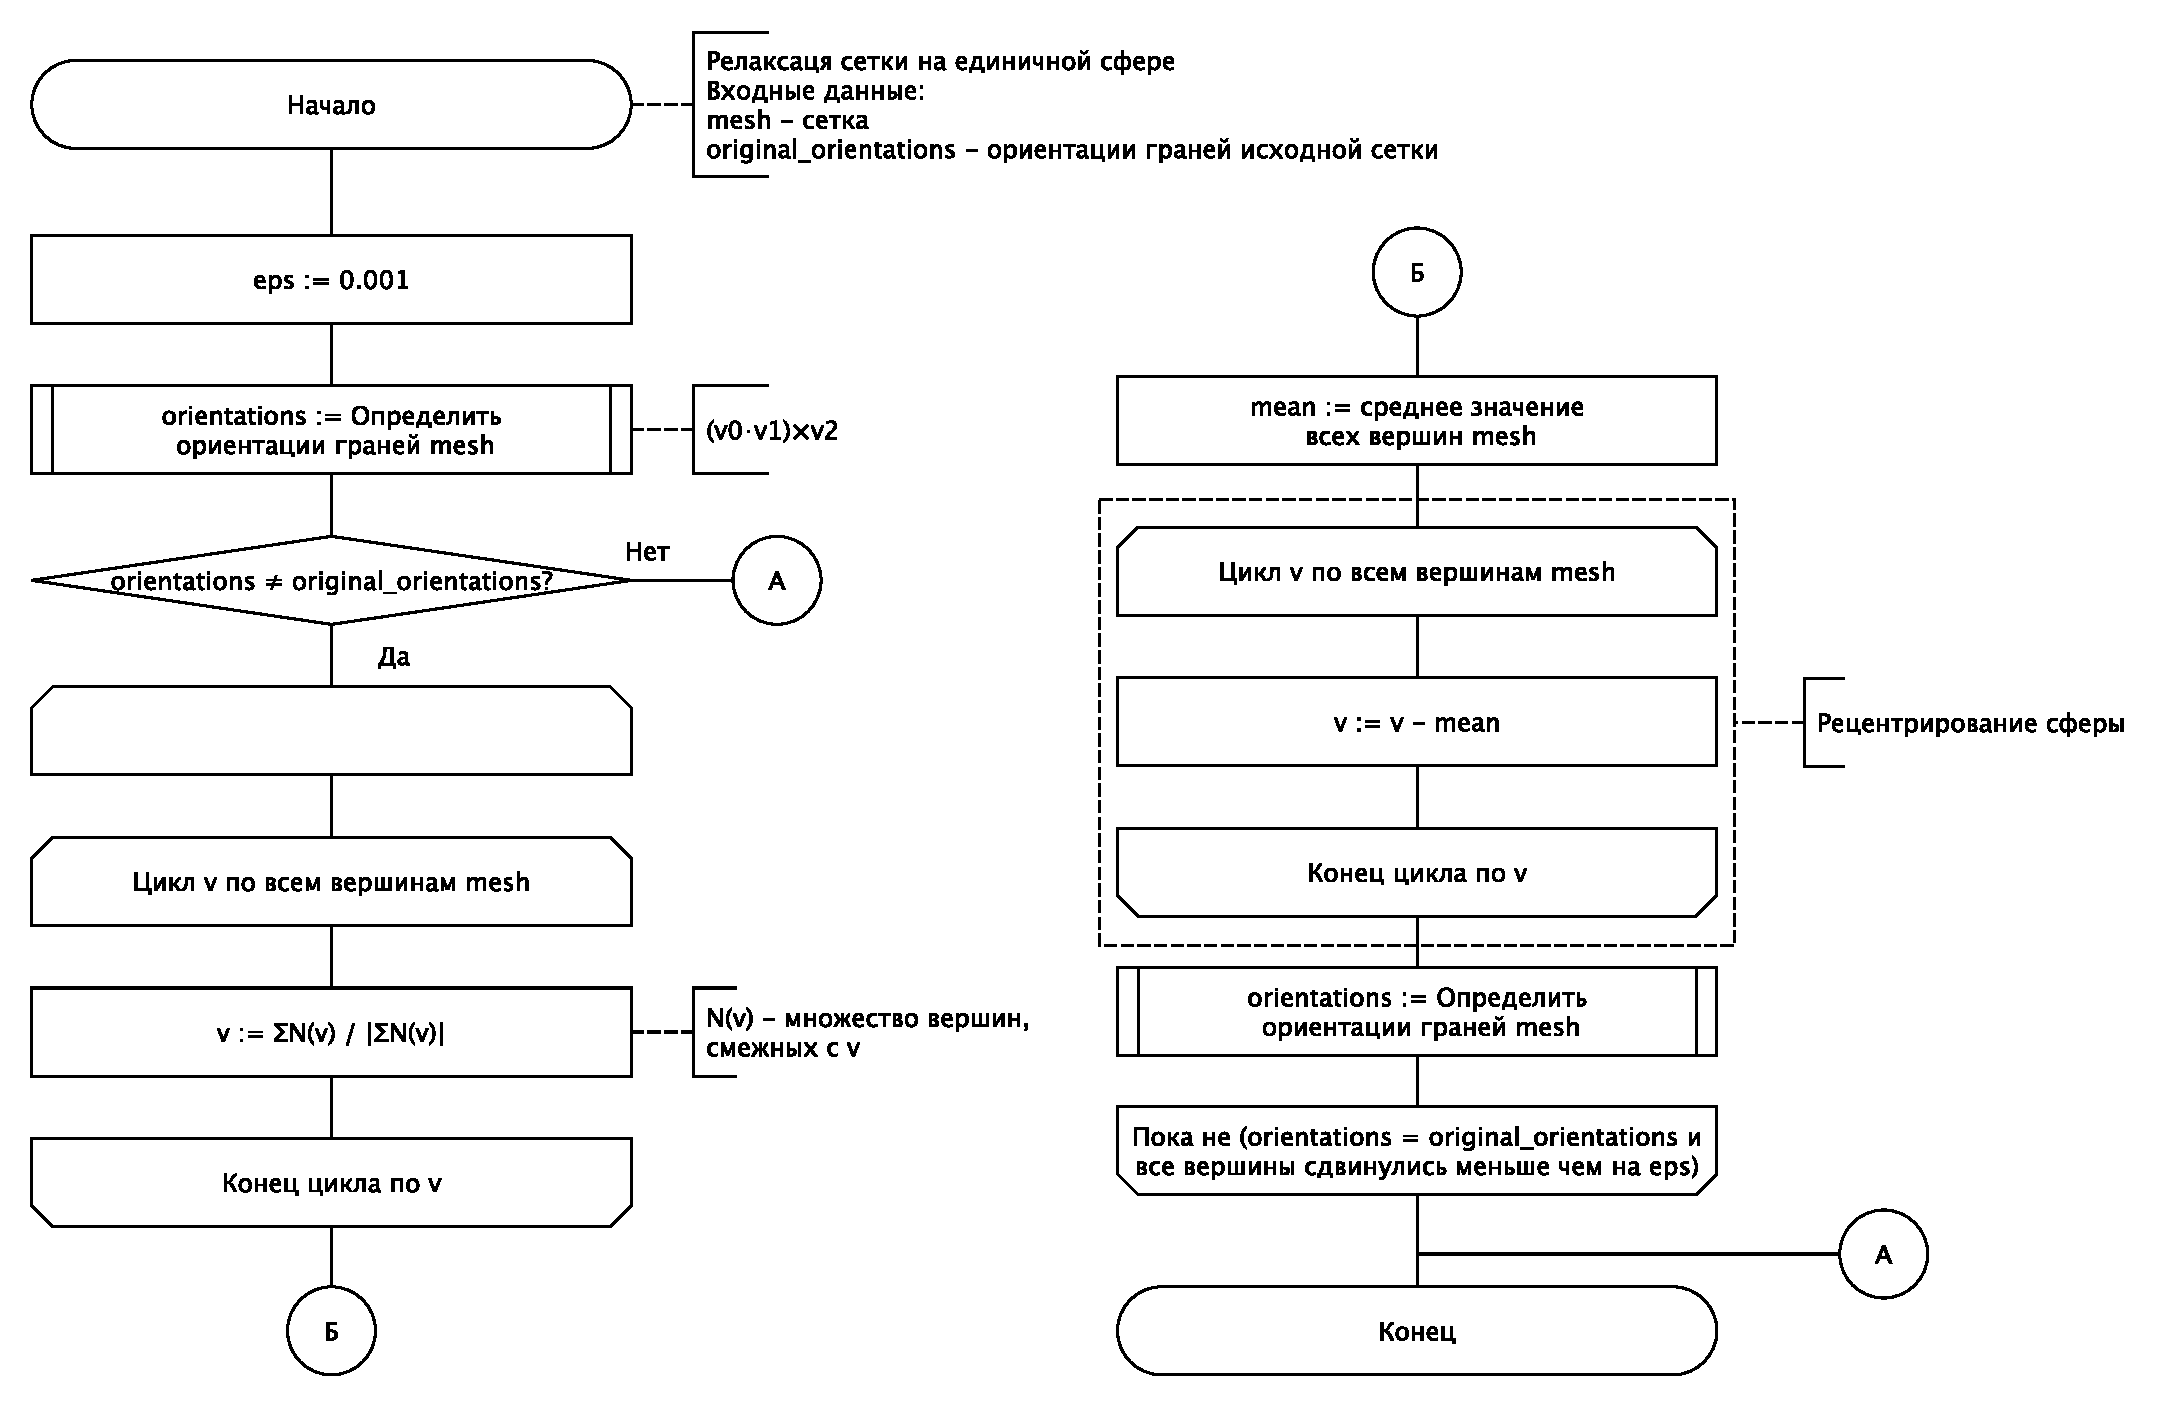
\includegraphics[width=\textwidth]{flowchart_relaxation}
	\caption{Схема алгоритма релаксации сетки}
\end{figure}

\begin{figure}[H]
	\label{fig:flowсhart_build_supermesh}
	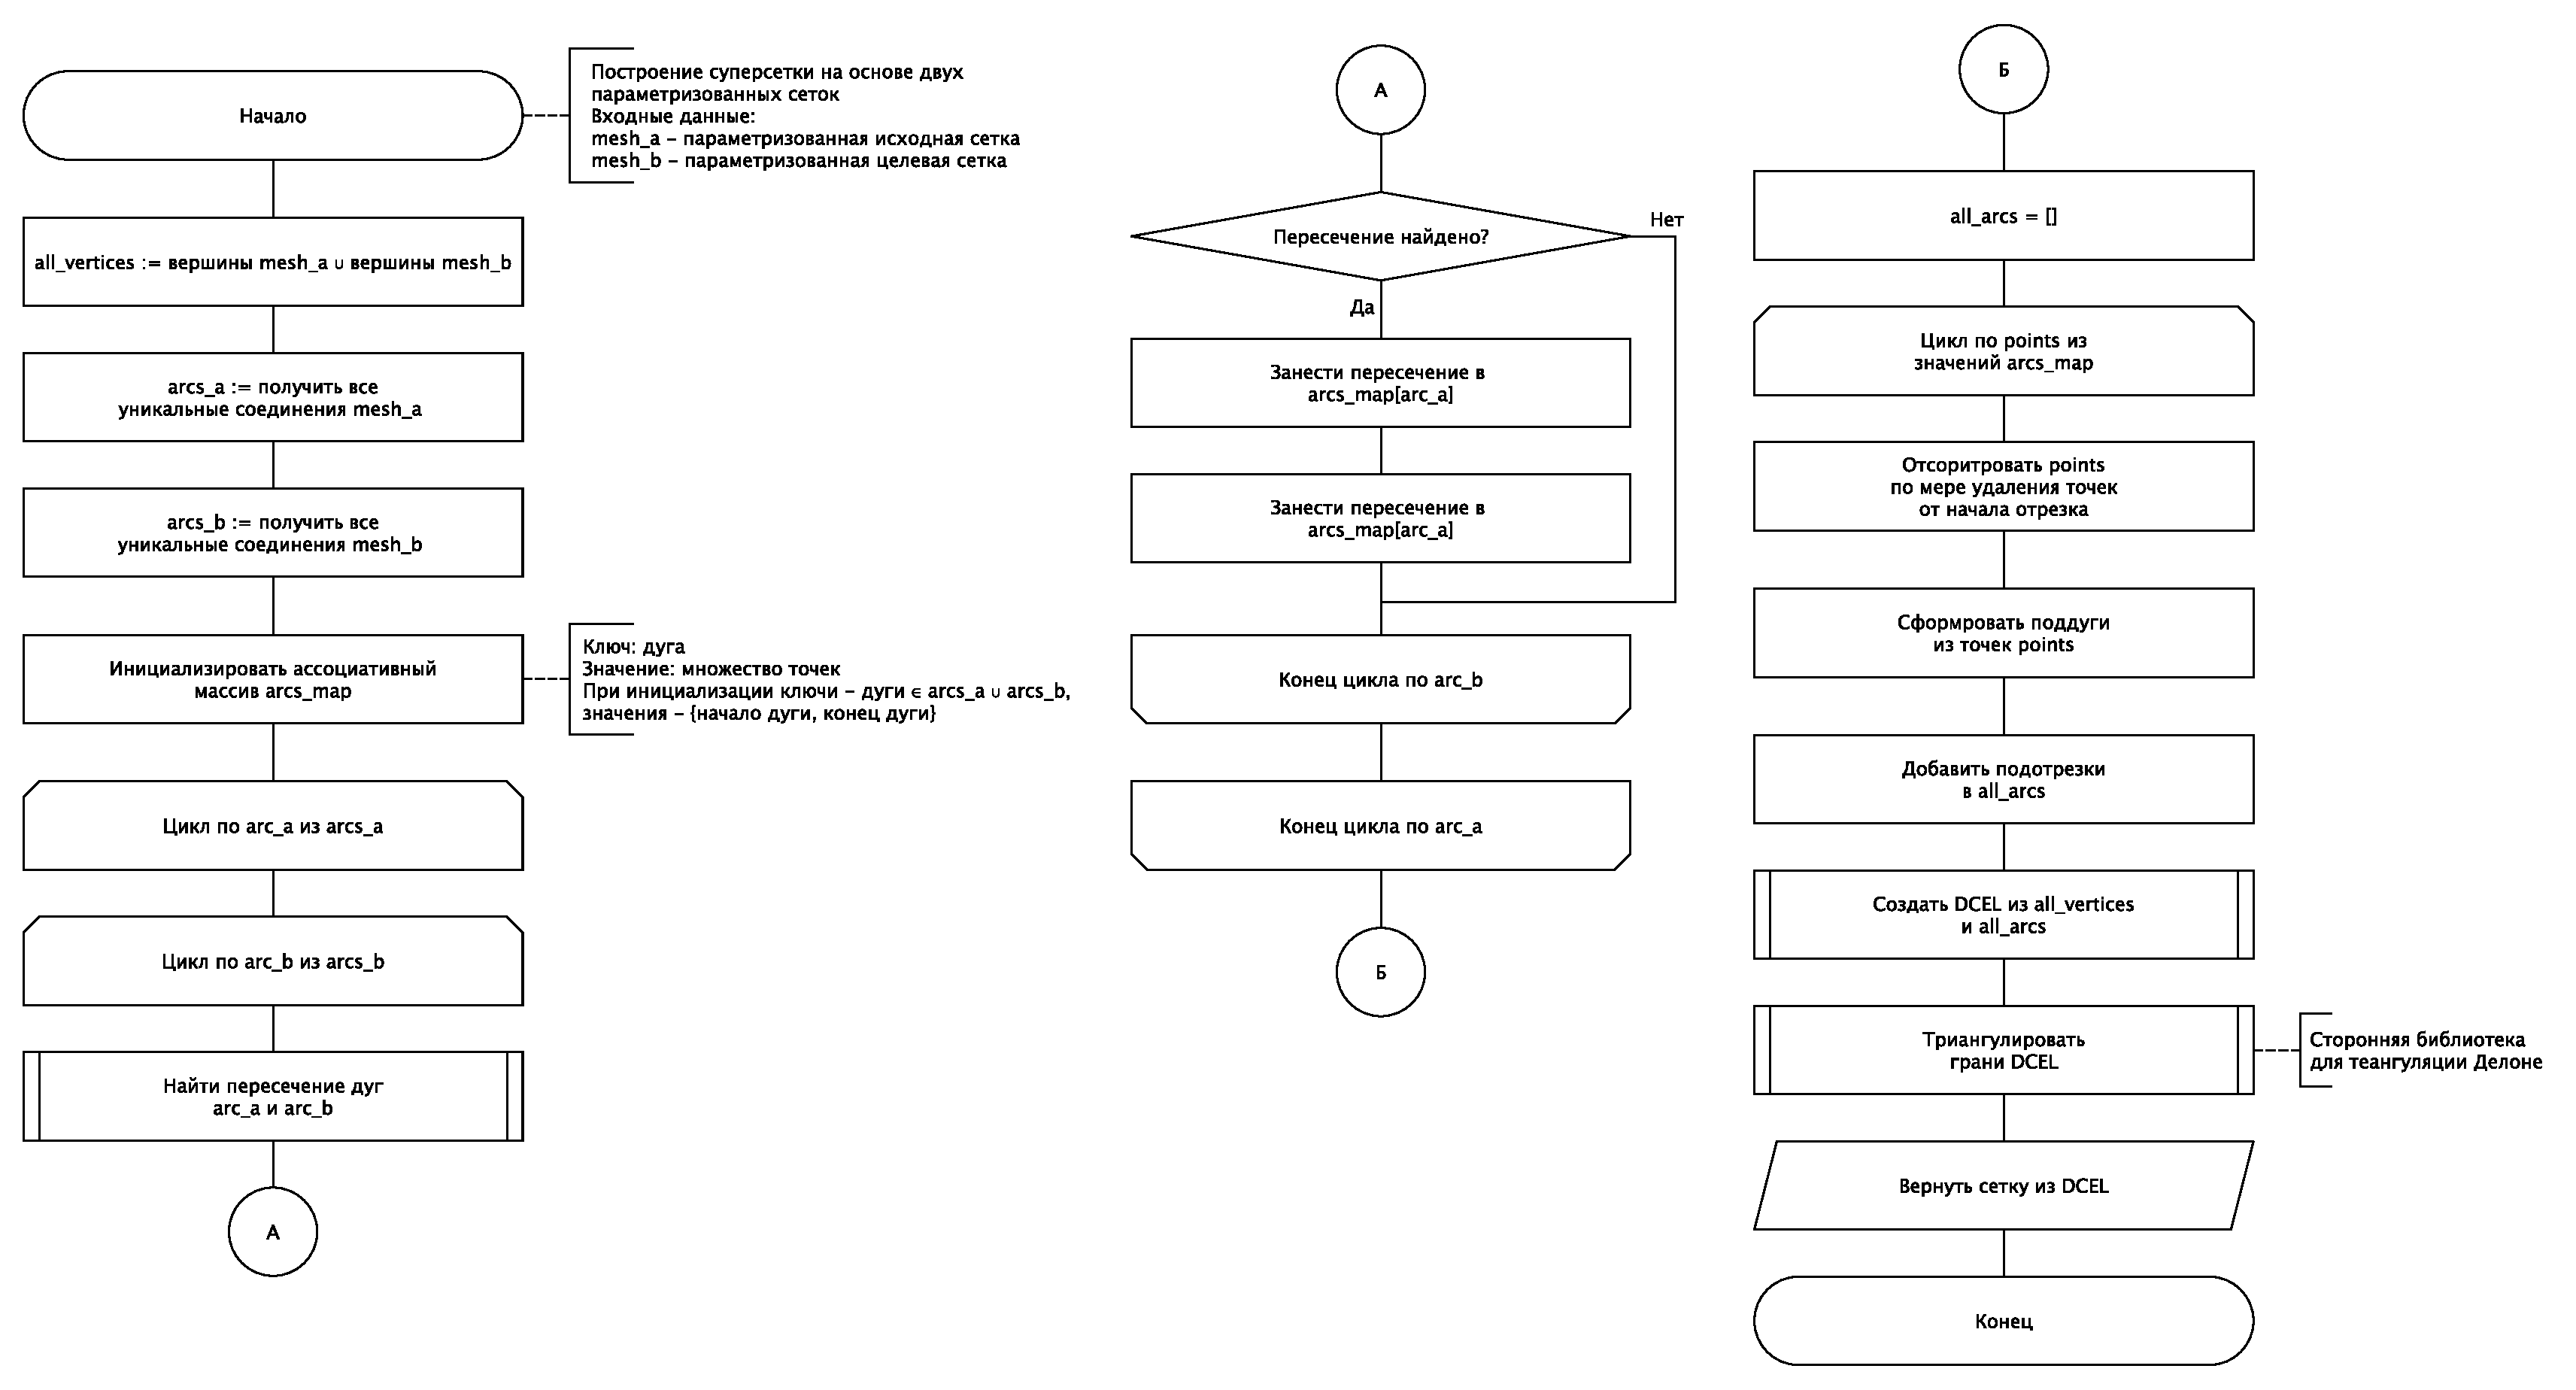
\includegraphics[width=\textwidth]{flowchart_bulid_supermesh}
	\caption{Схема алгоритма построения суперсетки на единичной сфере}
\end{figure}

\begin{figure}[H]
	\label{fig:flowсhart_vertex_relocation}
	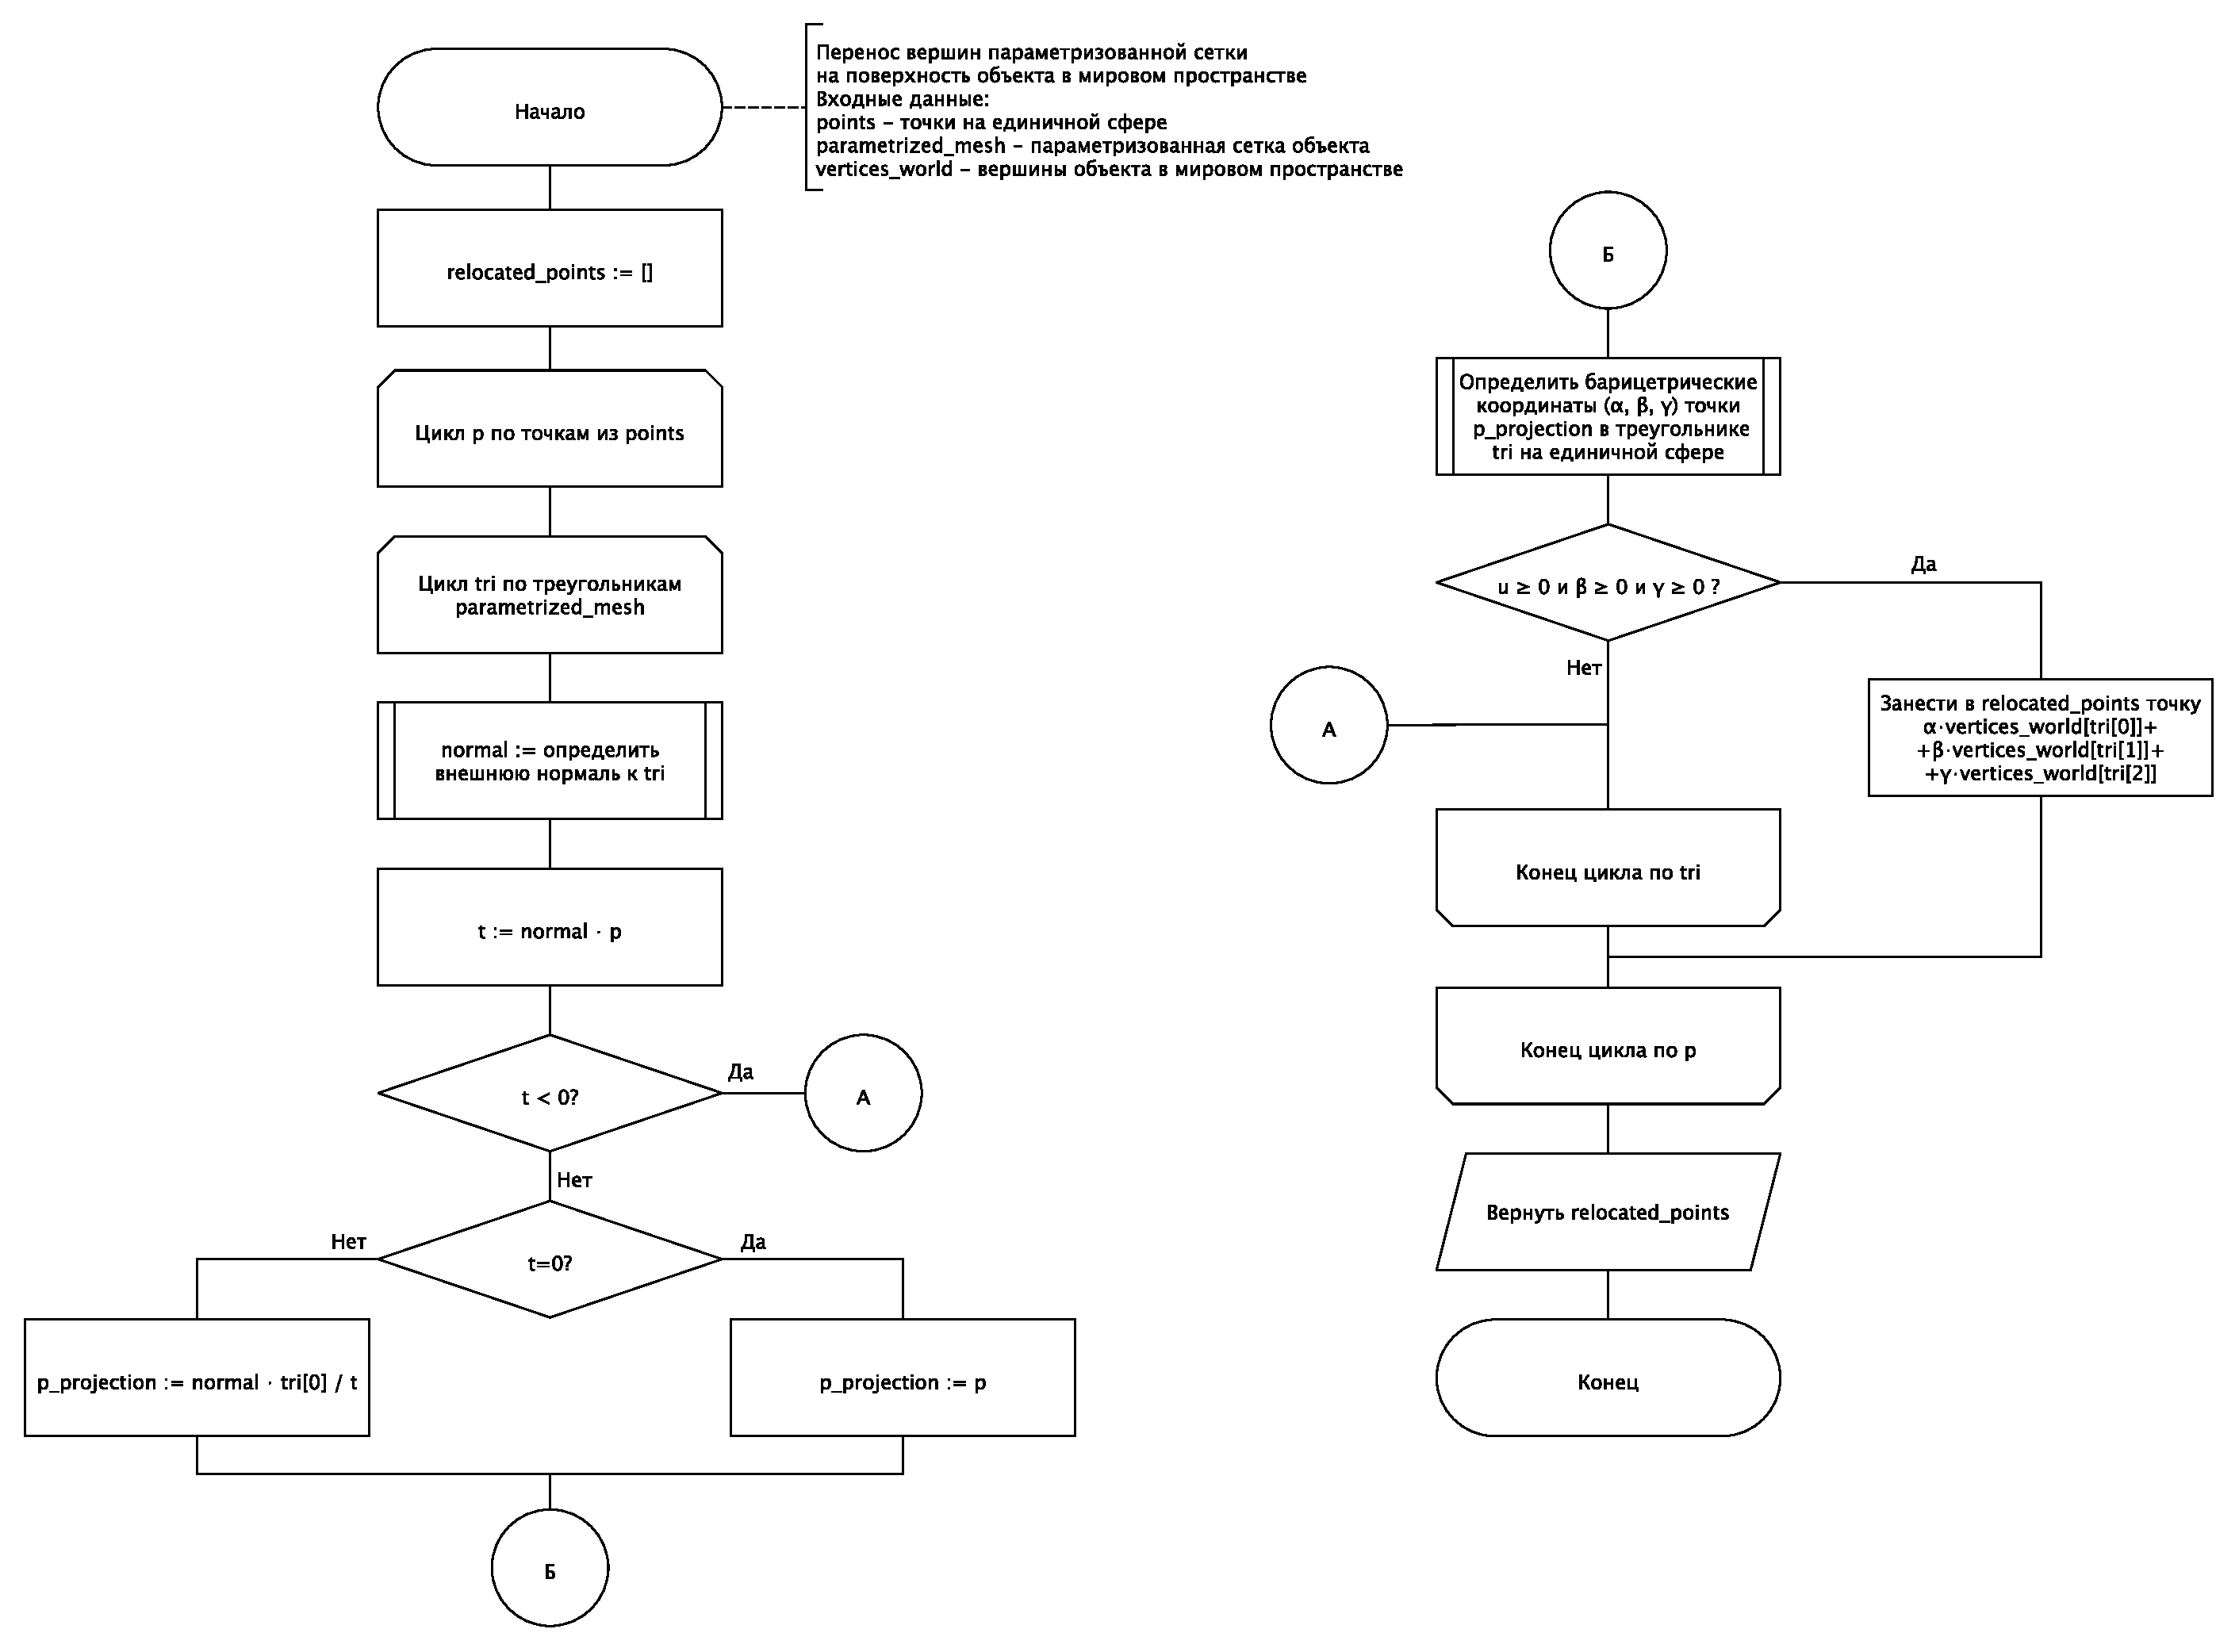
\includegraphics[width=\textwidth]{flowchart_vertex_relocation}
	\caption{Схема алгоритма переноса вершин суперсетки с единичной сферы в мировое пространство}
\end{figure}



\section*{Вывод}

\clearpage